\documentclass{article}
\usepackage[utf8]{inputenc}
\usepackage{amsmath}
\usepackage{amssymb}
\usepackage[hidelinks]{hyperref}
\usepackage{physics}
\usepackage{array} 
\usepackage{float}
\usepackage{cancel}
\usepackage{amsfonts}
\usepackage[italian]{babel}
\usepackage{mathrsfs}
\usepackage{mathtools}
\usepackage{yhmath}
\usepackage{amsthm}
\usepackage{caption}
\usepackage[rightcaption]{sidecap}
\usepackage{graphicx}
\usepackage{subfig}
\usepackage{lmodern}
\usepackage{bigints}
\usepackage{pgfplots}
\usepackage{bm}
\usepackage{textcomp}
\usepackage{siunitx}
\usepackage[a4paper, margin=0.8in]{geometry}
\usepackage{multirow}
\usepackage[utf8]{inputenc}
\usepackage{siunitx}

\usepackage[T1]{fontenc}
\usepackage[utf8]{inputenc}
\usepackage{babel}
\usepackage[font=small,labelfont=bf]{caption}


\begin{document}

\title{
  Laboratorio di Segnali e Sistemi - A.A. 2021/22 \\
  {\bf Esperienza 6:\\ 
  Elettronica digitale} \\}
\author{Chiara Scrocca 1855186 \\
Alessandro Tancredi 1919636 \\
        Rosso Vitale 1892051}
\maketitle
\date
\vspace{3cm}
\tableofcontents
\newpage
\section{Obiettivi dell'esperienza}
Lo'esperienza è sviluppata al fine di OIDDOCROP
    
\section{Apparato sperimentale}
    Per questa esperienza sono stati utilizzati:
    \begin{itemize}
        \item Generatore di segnali
        \item Generatore di tensione continua (elind MODEL 6TD20)
        \item Oscilloscopio digitale (Keysight DSOX1102G) con banda passante 70 MHz e frequenza di campionamento 2 GSa/s, impedenza d'ingresso 1 M$\Omega$ in parallelo a 16 pF.
        \item Breadboard 
        \item Multimetro da banco (Fluke 45) con risoluzione pari a 3\textperthousand, impedenza d'ingresso 10 M$\Omega$ in parallelo a $<$100 pF. 
        %\item Op-Amp LM358A (Fairchild Semiconductor)
        \item Integrato con gate NAND SN74LS00N Prodotto da Texas Instruments
    \end{itemize}
    
\section{Struttura dell'esperienza}
    L'esperienza è divisa in tre sezioni:
    \begin{enumerate}
        \item Realizzazione di un gate NOT e studio del suo comportamento
        \item Realizzazione di un gate XOR e studio del suo comportamento
        \item Realizzazione di un Flip-Flop SR e studio del suo comportamento
    \end{enumerate}
    \newpage
    \section{Gate NOT}
    Nella prima parte dell'esperienza è stato realizzato un gate NOT, come mostrato nella schematica in figura \ref{figNOT}, a partire da un gate NAND (La cui tabella di verità è la tabella \ref{tabTruthNAND}. Dopo aver assemblato e testato il circuito, ovvero dopo aver verificato che la tabella di verità associata (Tabella \ref{tabTruthNOT}) a tale gate logico fosse rispettata, sono stati registrati i valori di $V_{in}$ e $V_{out}$, realizzando il grafico mostrato in figura \ref{figNotGraf}.
    
    
    \begin{table}[H]
    \centering
        \begin{minipage}[b]{0.32\hsize}\centering
            \begin{tabular}{ | c | c |}
               \hline
               A & Q \\ \hline \hline
               0 & 1 \\ \hline
               1 & 0 \\ \hline
            \end{tabular}
            \caption{Tabella verità NOT}
            \label{tabTruthNOT}
        \end{minipage}
        %\hfill
        \begin{minipage}[b]{0.32\hsize}\centering
            \begin{tabular}{ | c | c | c |}
               \hline
               A & B & Q \\ \hline \hline
               0 & 0 & 1 \\ \hline
               0 & 1 & 1 \\ \hline
               1 & 0 & 1 \\ \hline
               1 & 1 & 0 \\ \hline
            \end{tabular}
            \caption{Tabella verità NAND}
            \label{tabTruthNAND}
        \end{minipage}
    \end{table}
    
    
    \begin{figure}[H]
        \minipage{0.5\textwidth}
          \centering
          \includegraphics[width=0.9\linewidth]{Images/Schematicanot.png}
          \caption{Schematica circuitale per il gate NOT}
          \label{figNOT}
        \endminipage
        \hspace{0.7cm}
        \minipage{0.5\textwidth}
          \centering
          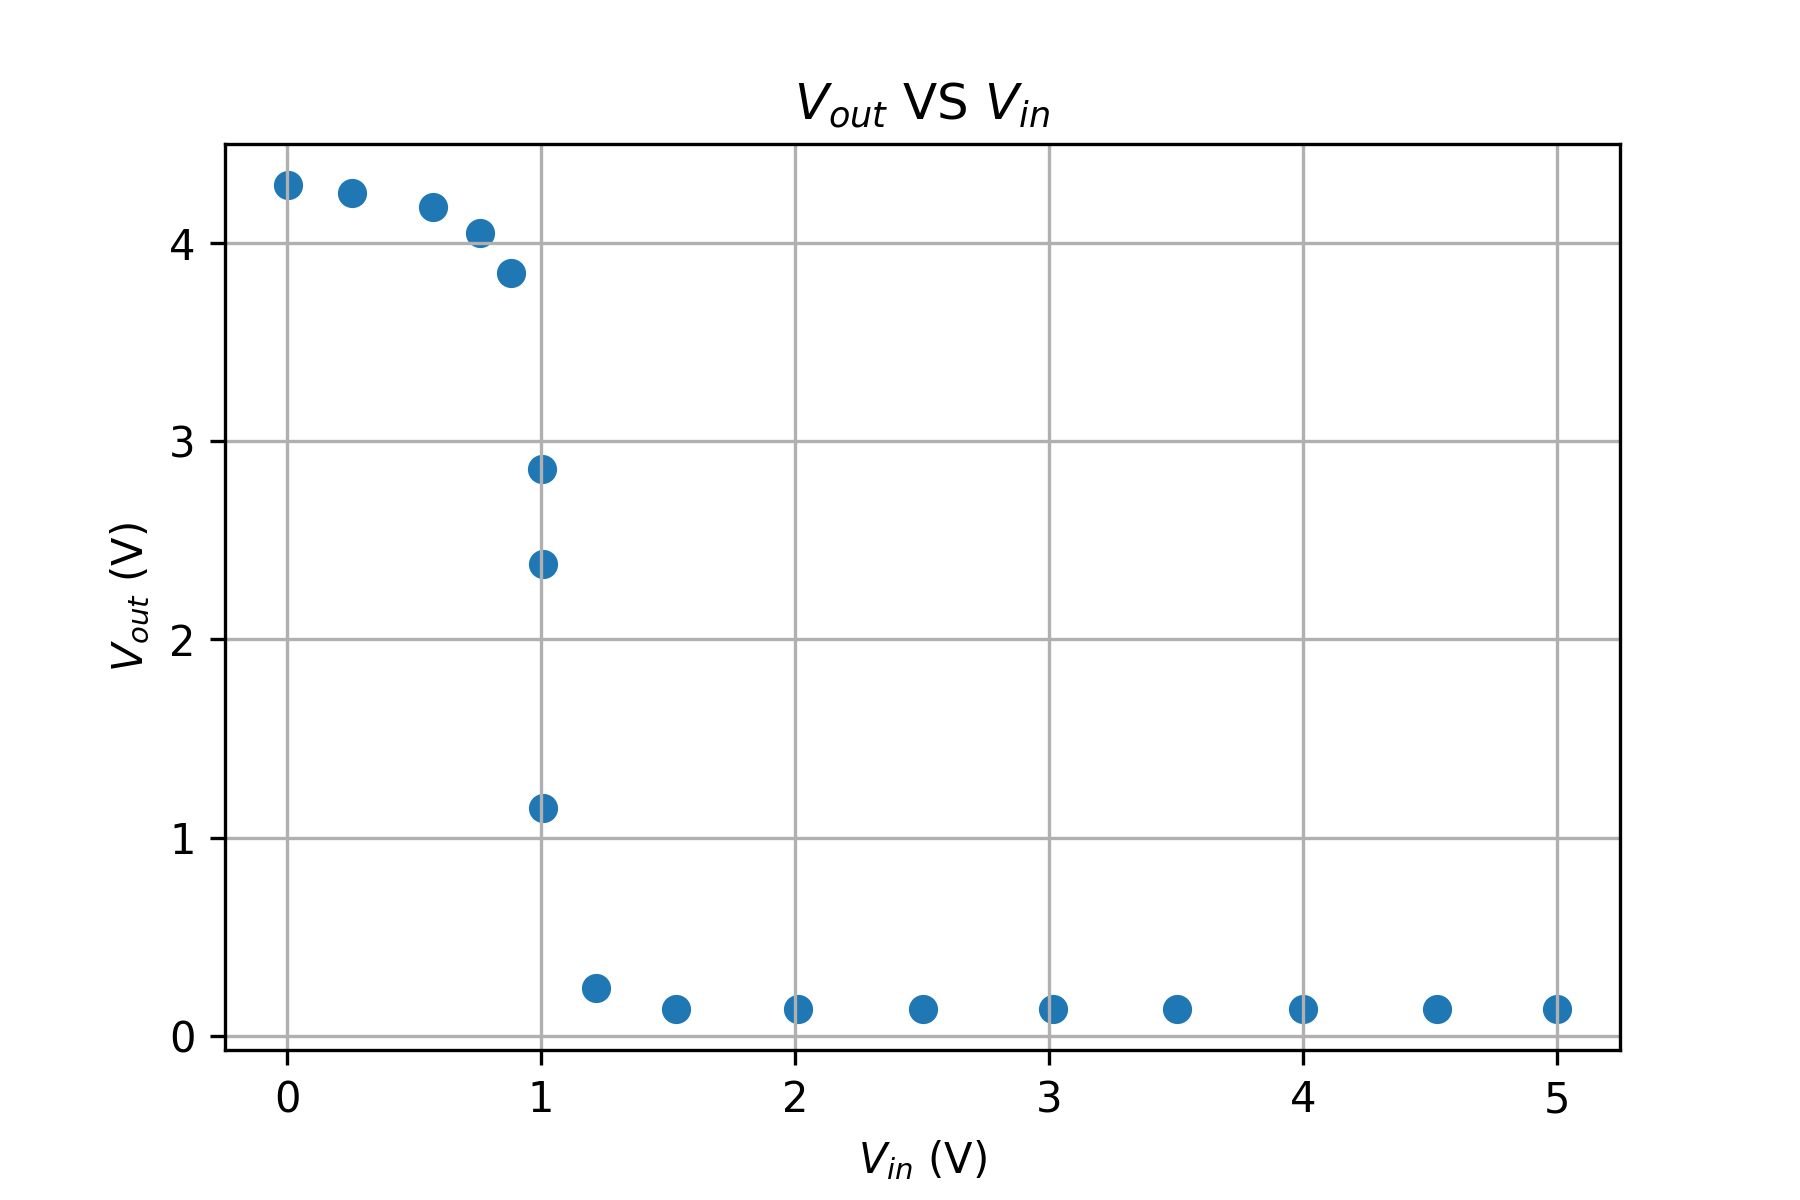
\includegraphics[width=0.9\linewidth]{Images/Not.png}
          \caption{Grafico prodotto dai dati raccolti}
          \label{figNotGraf}
        \endminipage\hfill
    \end{figure}
        
    A partire dai dati raccolti, riportati in tabella \ref{MADONNTROIA}, è stata stimata la tensione di transizione da uno stato logico all'altro, pari a $V_T = (1.XX\pm YY)V$.
    Si è quindi proceduto a testare tutte le porte logiche dell'integrato, al fine di verificarne il funzionamento.
    
    Per visualizzare sull'oscilloscopio il comportamento del gate realizzato, è stato utilizzato come segnale d'ingresso un'onda triangolare di ampiezza pari a $\Delta V=(5.00\pm0.15)V$ e con un offset di $V_{off}=(2.500\pm0.004)V$, osservando il risultato mostrato in figura \ref{figNotOsc}.
    \begin{figure}[H]
        \centering
        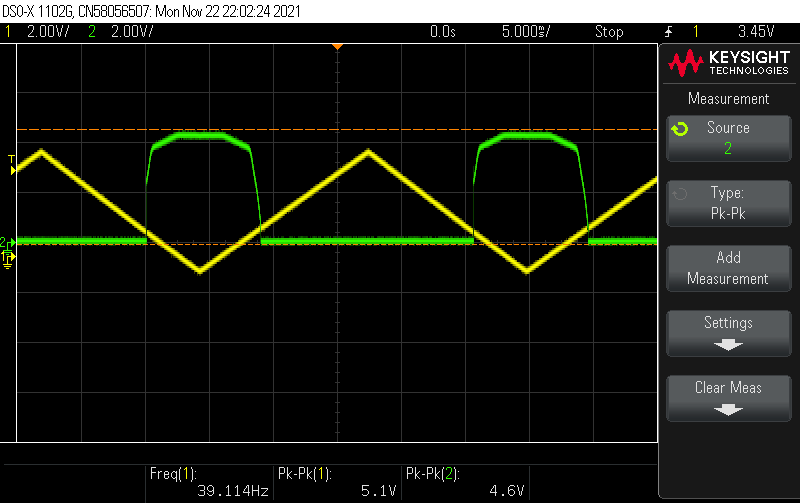
\includegraphics[scale=0.35]{Images/scope_5.png}
        \caption{Vista all'oscilloscopio}
        \label{figNotOsc}
    \end{figure}

    \begin{table}[]
        \centering
        \begin{tabular}{c|c}
             &  \\
             & 
        \end{tabular}
        \caption{Caption}
        \label{MADONNATROIA}
    \end{table}
\newpage

\section{Gate XOR}
    In questa parte dell'esperienza è stato realizzato un gate XOR, in accordo con la schematica \ref{figXORSchem}. Dopo aver assemblato il circuito è stato verificato che esso si comportasse come descritto dalla tabella di verità associata (\ref{tabTruthXOR}).
  
    \begin{minipage}{\textwidth}
    \begin{minipage}[b]{0.49\textwidth}
        \centering
        \includegraphics[scale=0.8]{Images/ScemXOR.png}
        \captionof{figure}{Schematica del circuito con XOR}
        \label{figXORSchem}
    \end{minipage}
    \hfill
    \begin{minipage}[b]{0.49\textwidth}
        \centering
        \begin{tabular}{ | c | c | c |}
           \hline
           A & B & Q \\ \hline \hline
           0 & 0 & 0 \\ \hline
           0 & 1 & 1 \\ \hline
           1 & 0 & 1 \\ \hline
           1 & 1 & 0 \\ \hline
        \end{tabular}
        \captionof{table}{Tabella di verità XOR}
        \label{tabTruthXOR}
        \end{minipage}
    \end{minipage}
    \vspace{1cm}
    
    Per avere una visualizzazione più veloce e chiara degli stati logici di ingressi e uscita, sono stati utilizzati del LED: due led verdi per i segnali d'ingresso e un led rosso per l'uscita. Nella foto del circuito (figura \ref{CircXOR}) è possibile vedere come i LED sono stati montati, per poter comprendere le immagini successive.
    Per utiizzare i LED, essi sono stati protetti da dei resistori di resistenza $R\approx330\Omega$ e collegati secondo la giusta polarità.
    
    
    
    \begin{figure}[H]
    \captionsetup{labelformat=empty}
    \minipage{0.5\textwidth}
      \centering
      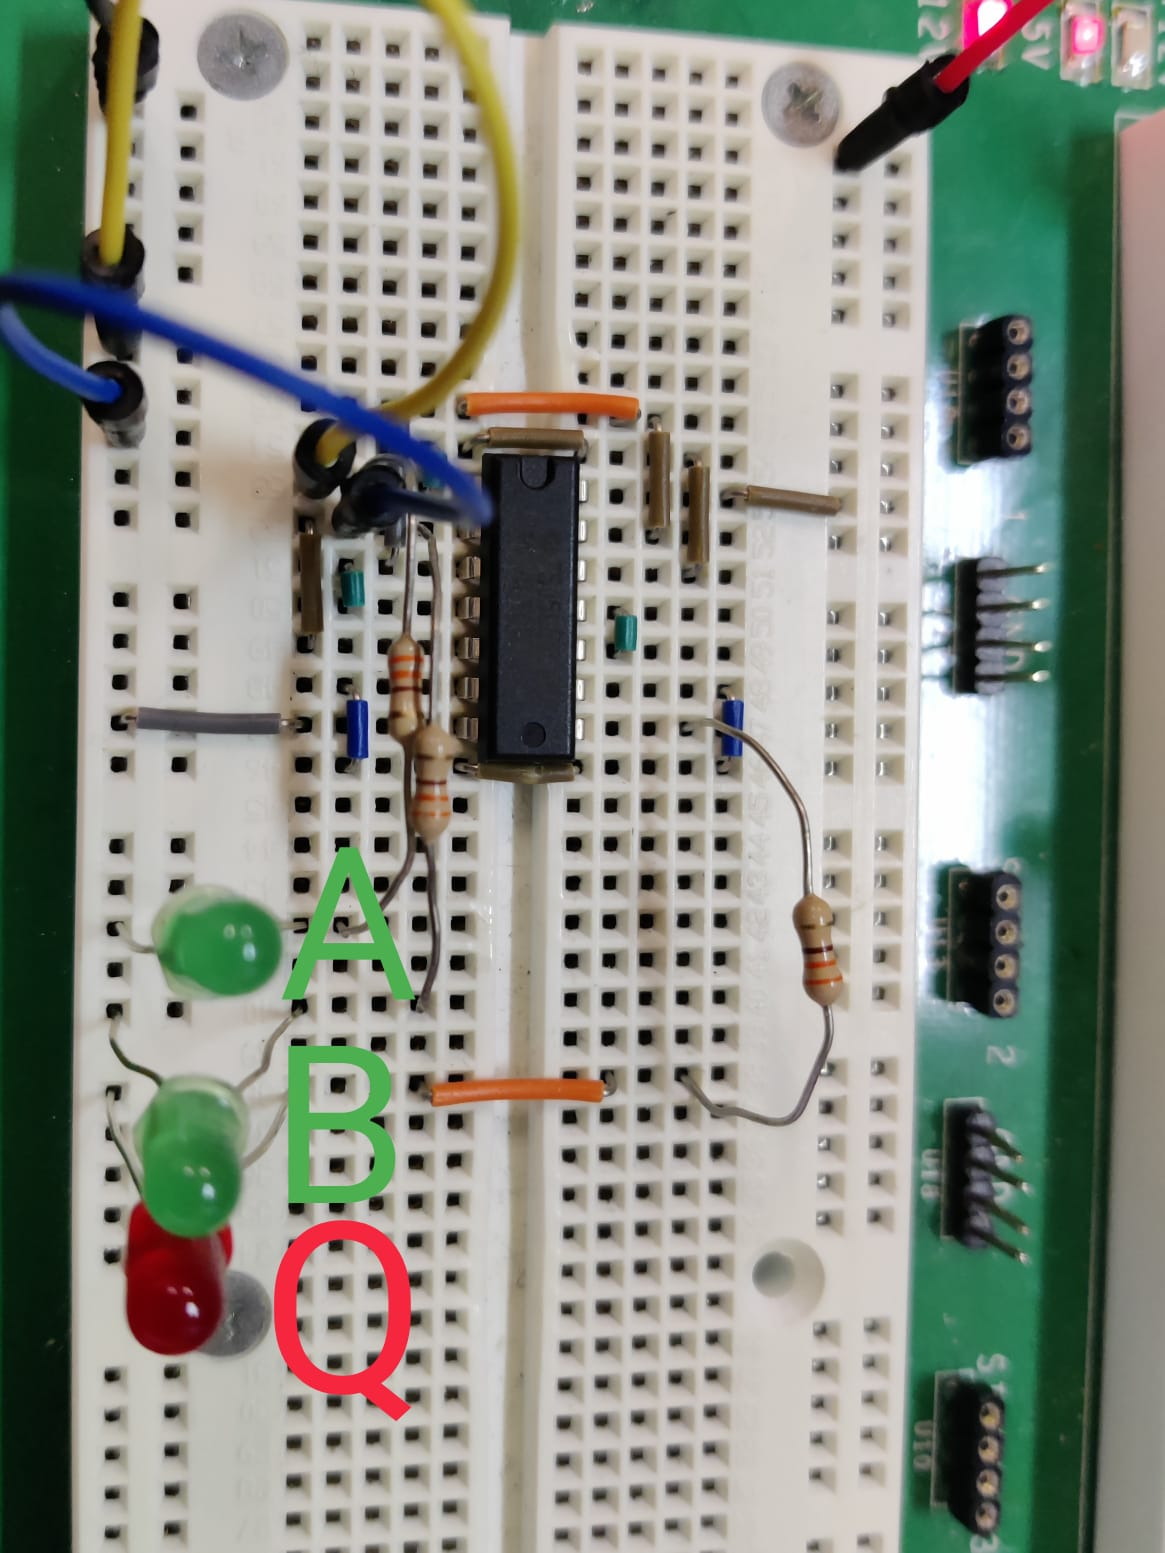
\includegraphics[width=0.5\linewidth]{Images/XOR_0.jpeg}
      \caption{Configurazione 0 0 0}
    \endminipage
    \hspace{0.7cm}
    \minipage{0.5\textwidth}
      \centering
      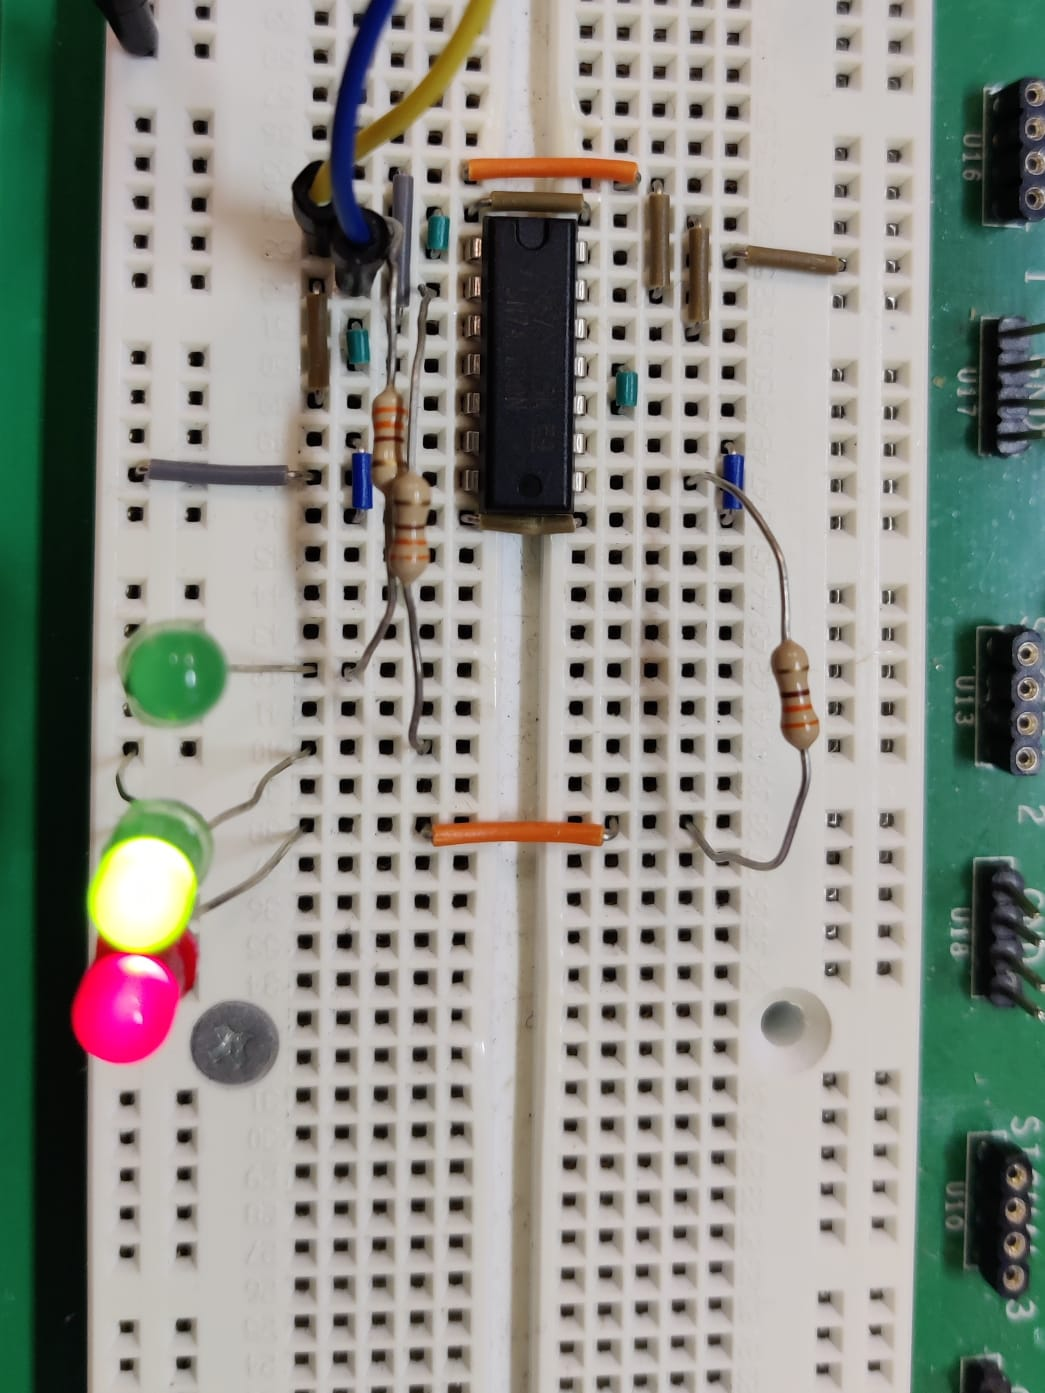
\includegraphics[width=0.5\linewidth]{Images/XOR_2.jpeg}
      \caption{Configurazione 0 1 1}
    \endminipage\hfill
    \minipage{0.5\textwidth}
     \centering
      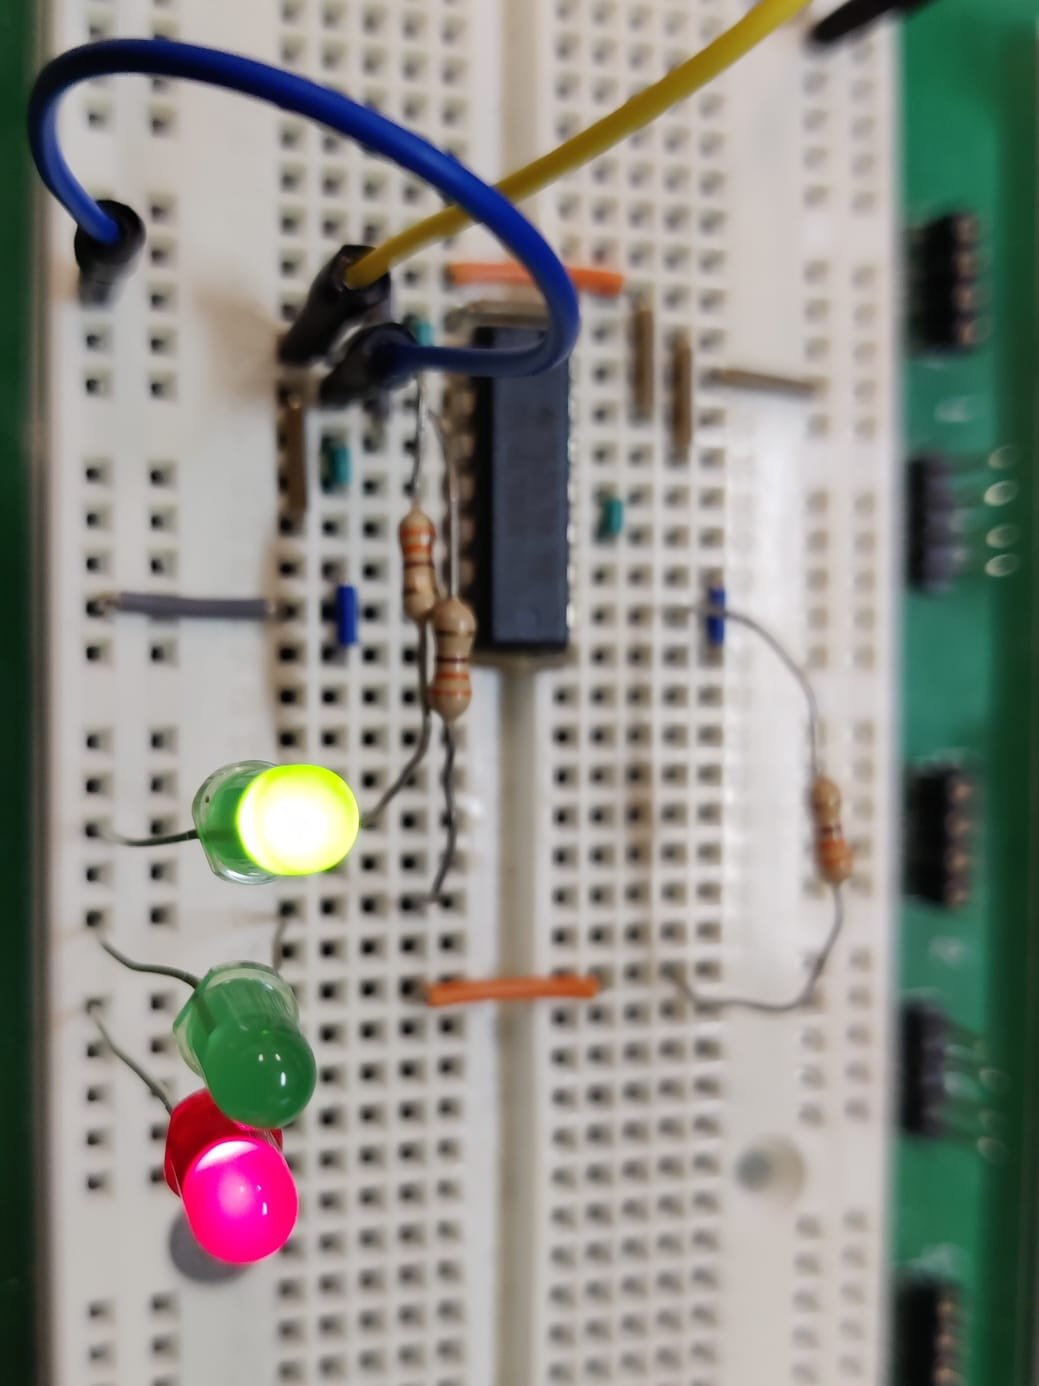
\includegraphics[width=0.5\linewidth]{Images/XOR_1.jpeg}
      \caption{Configurazione 1 0 1}
    \endminipage
    \hspace{0.7cm}
    \minipage{0.5\textwidth}
     \centering
      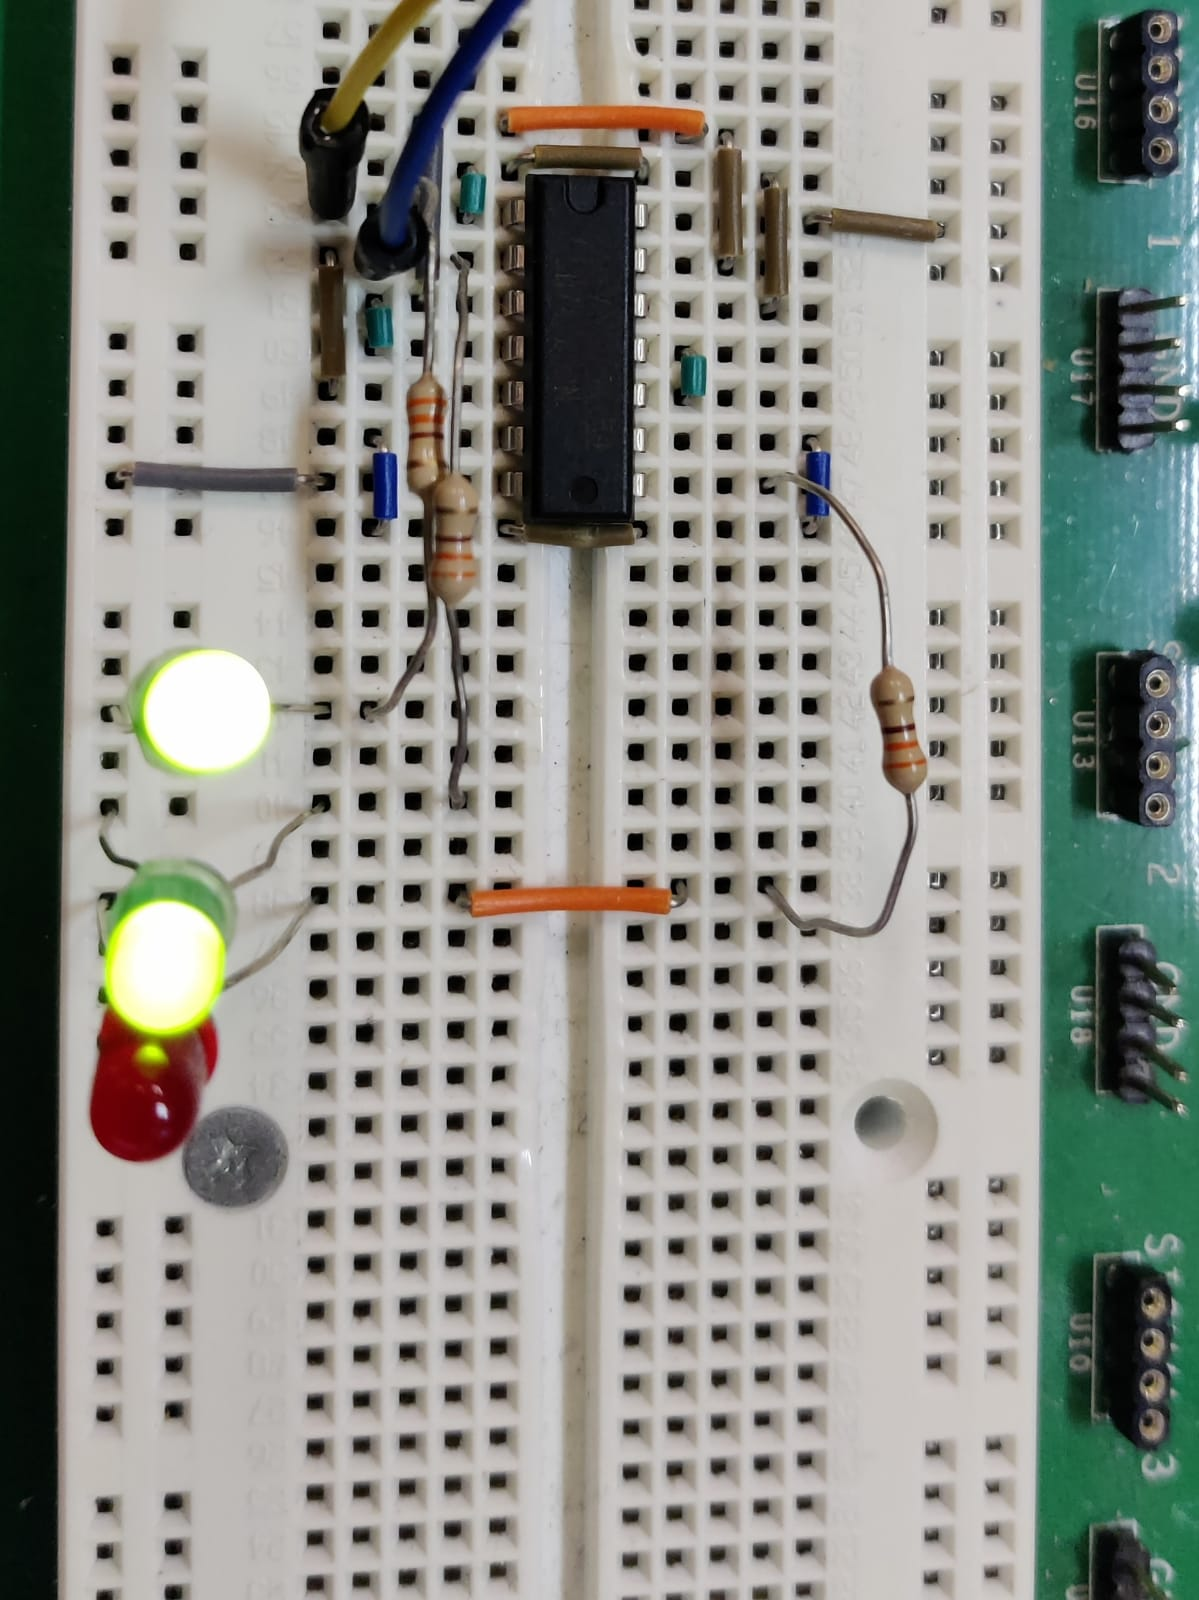
\includegraphics[width=0.5\linewidth]{Images/XOR_3.jpeg}
      \caption{Configurazione 1 1 0}
    \endminipage\hfill
    \caption{Combinazioni possibili nell'utilizzo del gate XOR}
    \end{figure}
    
    Un'ulteriore verifica è stata effettuata misurando le tensioni d'uscita e d'ingresso con il multimetro, ottenendo conferma di quanto dedotto visivamente, in particolare misurando valori sempre maggiori di $V_{min}=3.3V$ per gli stati \textbf{True} e valori sempre inferiori a $V_{max}=200mV$ per gli stati \textbf{False}.
    
    Una volta effettuate tali verifiche e dimostrato quindi il corretto funzionamento del circuito, ponendo l'ingresso A prima su \textbf{True} e poi su \textbf{False}, e mandando in B un'onda quadra di ampiezza $\Delta V = (5\pm0.15)V$ e con un offset di $V_{off}=(2.500\pm0.004)V$ è stato possibile osservare l'andamento prima in opposizione di fase e poi in fase dell'uscita Q con il segnale B. È possibile osservare tale fenomenologia in figure \ref{XORA1} e \ref{XORA0}.
    
    \begin{figure}[H]
        \minipage{0.5\textwidth}
          \centering
          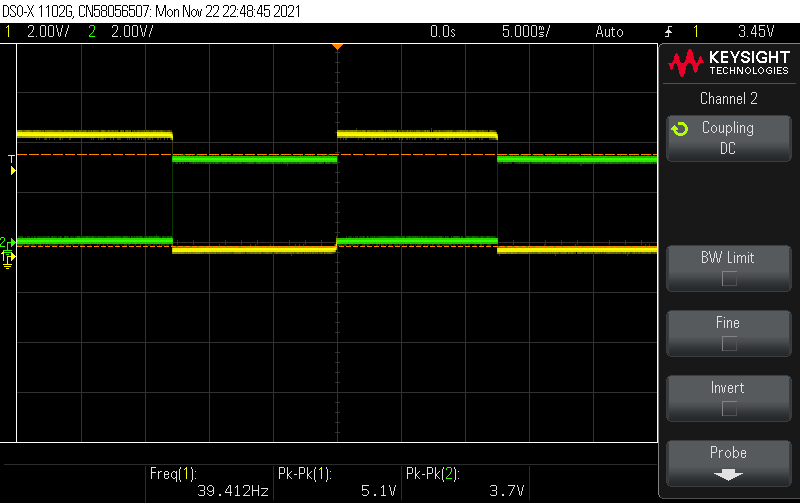
\includegraphics[width=0.9\linewidth]{Images/scope_7.png}
          \caption{Andamento di Q con A impostato come \textbf{True}}
          \label{XORA1}
        \endminipage
        \hspace{0.7cm}
        \minipage{0.5\textwidth}
          \centering
          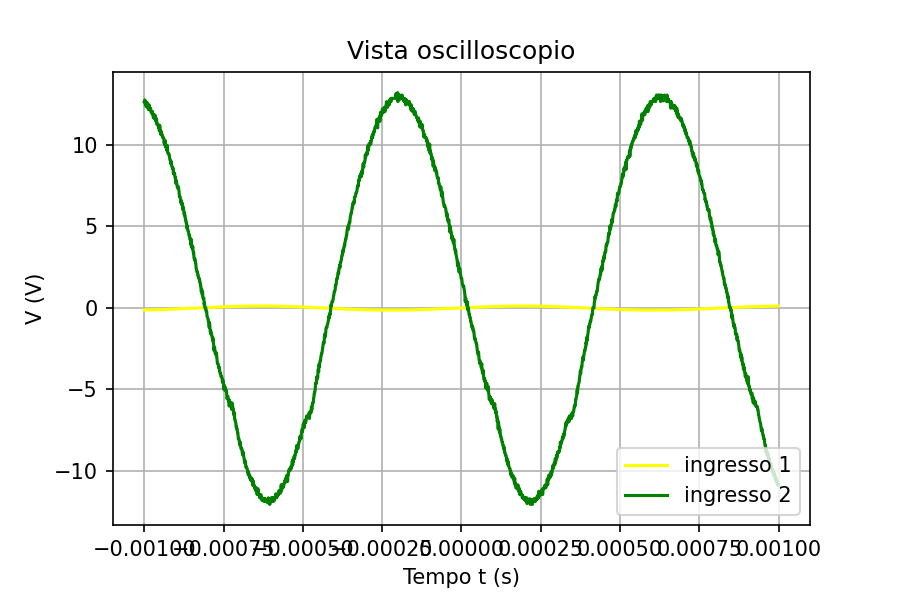
\includegraphics[width=0.9\linewidth]{Images/scope_8.png}
          \caption{Andamento di Q con A impostato come \textbf{False}}
          \label{XORA0}
        \endminipage\hfill
    \end{figure}
    
    
    
\section{Flip-Flop SR}
    Per questa sezione dell'esperienza è stato assemblato un circuito logico Flip-Flop SR, come mostratio nella figura \ref{figFFSR}, si è quindi proceduto a verificarne il corretto funzionamento, descritto dalla tavola di verità \ref{TVFF}.
    
\section{Conclusioni}
    Stocazzo
 
\end{document}
